%%%%%%%%%%%%%%%%%%%%%%%%%%%%%%%%%%%%%%%%%%%%%%%%%%%%%%%%%%%%%%%%%%%%%%%%
%   LaTeX source code to approximate a NIST Technical report
%	Instructions for authors: tinyurl.com/techpubsnist 
%	DOI watermark will be added on final PDF
% 	Developed by K. Miller, kmm5@nist.gov 
%	Last updated: 22-January-2021
%%%%%%%%%%%%%%%%%%%%%%%%%%%%%%%%%%%%%%%%%%%%%%%%%%%%%%%%%%%%%%%%%%%
\documentclass[12pt]{article}
\usepackage{amsmath}
\usepackage{amsfonts}   % if you want the fonts
\usepackage{amssymb}    % if you want extra symbols
\usepackage{graphicx}   % need for figures
\usepackage{xcolor}
\usepackage{caption}
\usepackage{bm}
\usepackage{secdot}	
\usepackage{listings}	
\usepackage{mathptmx}
\usepackage{float}
\usepackage[utf8]{inputenc}
\usepackage{textcomp}
\usepackage[hang,flushmargin,bottom]{footmisc} % footnote format
\setlength{\parindent}{0pt}

% colori per il codice

\definecolor{codegreen}{rgb}{0,0.6,0}
\definecolor{codegray}{rgb}{0.5,0.5,0.5}
\definecolor{codepurple}{rgb}{0.58,0,0.82}
\definecolor{backcolour}{rgb}{0.95,0.95,0.92}

\lstdefinestyle{mystyle}{
    backgroundcolor=\color{backcolour},   
    commentstyle=\color{codegreen},
    keywordstyle=\color{magenta},
    numberstyle=\tiny\color{codegray},
    stringstyle=\color{codepurple},
    basicstyle=\ttfamily\footnotesize,
    breakatwhitespace=false,         
    breaklines=true,                 
    captionpos=b,                    
    keepspaces=true,                 
    numbers=left,                    
    numbersep=5pt,                  
    showspaces=false,                
    showstringspaces=false,
    showtabs=false,                  
    tabsize=2
}

\lstset{style=mystyle}

\usepackage{titlesec}
\titleformat{\section}{\normalsize\bfseries}{\thesection.}{1em}{}	% required for heading numbering style
\titleformat*{\subsection}{\normalsize\bfseries}

\usepackage{tocloft}	% change typeset, titles, and format list of appendices/figures/tables
\renewcommand{\cftdot}{}	
\renewcommand{\contentsname}{Table of Contents}
\renewcommand{\cftpartleader}{\cftdotfill{\cftdotsep}} % for parts
\renewcommand{\cftsecleader}{\cftdotfill{\cftdotsep}}
\renewcommand\cftbeforesecskip{\setlength{4pt}{}}
\addtolength{\cftfignumwidth}{1em}
\renewcommand{\cftfigpresnum}{\figurename\ }
\addtolength{\cfttabnumwidth}{1em}
\renewcommand{\cfttabpresnum}{\tablename\ }
\setlength{\cfttabindent}{0in}    %% adjust as you like
\setlength{\cftfigindent}{0in} 

\usepackage{enumitem}         % to control spacing between bullets/numbered lists

% \usepackage[numbers,sort&compress]{natbib} % format bibliography 
% \renewcommand{\bibsection}{}
% \setlength{\bibsep}{20.0pt}

\usepackage[hidelinks]{hyperref}
\hypersetup{
	colorlinks = true,
urlcolor ={blue},
citecolor = {.},
linkcolor = {.},
anchorcolor = {.},
filecolor = {.},
menucolor = {.},
runcolor = {.}
pdftitle={},%%put title here to auto-fill properties of the PDF
pdfsubject={},%%put abstract here
pdfauthor={}, %%put author list here
pdfkeywords={} %%put keywords here
}
\urlstyle{same}

\usepackage{epstopdf} % converting EPS figure files to PDF

\usepackage{fancyhdr, lastpage}	% formatting document, calculating number of pages, formatting headers
\setlength{\topmargin}{-0.5in}
\setlength{\headheight}{39pt}
\setlength{\oddsidemargin}{0.25in}
\setlength{\evensidemargin}{0.25in}
\setlength{\textwidth}{6.0in}
\setlength{\textheight}{8.5in}

\usepackage{caption} % required for Figure labels
\captionsetup{font=small,labelfont=bf,figurename=Fig.,labelsep=period,justification=raggedright} 

%%%%%%%%%%% !!!!!! REQUIRED - FILL OUT METADATA HERE !!!!!!!! %%%%%%%%%%%%%%
%  	Report Number - fill in Report Number sent to you (see info below)
%   DOI Statement - fill in DOI sent to you 
%   Month Year - fill in Month and Year of Publication
%%%%%%%%%%%%%%%%%%%%%%%%%%%%%%%%%%%%%%%%%%%%%%%%%%%%%%%%%%%%%%%%%%%%%%%%%%%%%%%%%%%%%%
\newcommand{\pubnumber}{1500-XX}
\newcommand{\DOI}{https://doi.org/10.6028/NIST.SP.1500-XX}
\newcommand{\monthyear}{Month Year}
%%%%%%%%%%%%%%%%%%%%%%%%%%%%%%%%%%%%%%%%%%%%%%%%%%%%%%%%%%%%%%%%%%%%
%   	BEGIN DOCUMENT 
%%%%%%%%%%%%%%%%%%%%%%%%%%%%%%%%%%%%%%%%%%%%%%%%%%%%%%%%%%%%%%%%%%%%
\begin{document}
\urlstyle{rm} % Format style of \url   

%%%%%%%%%%%%%%%%%%%%%%%%%%%%%%%%%%%%%%%%%%%%%%%%%%%%%%%%%%%%%%%%%%%%
%   Cover Page is REQUIRED and must contain the information 
%	displayed here, at a minimum. Additional artwork may be included 
%	(e.g., official project/conference logo, etc.).
%	Pub Number automated based on metadata
%%%%%%%%%%%%%%%%%%%%%%%%%%%%%%%%%%%%%%%%%%%%%%%%%%%%%%%%%%%%%%%%%%%%
\begin{titlepage}
    \begin{flushright}
        %%%%%%%%%%%%%%%%%%%%%%%%%%%%%%%%%%%%%%%%%%%%%%%%%%%%%%%%%%%%%%%%%%%%
        % 	Automated based on metadata - delete if not applicable
        %%%%%%%%%%%%%%%%%%%%%%%%%%%%%%%%%%%%%%%%%%%%%%%%%%%%%%%%%%%%%%%%%%%%
        \LARGE{\textbf{Molecular Simulations Report}}\\
        \vfill
        %%%%%%%%%%%%%%%%%%%%%%%%%%%%%%%%%%%%%%%%%%%%%%%%%%%%%%%%%%%%%%%%%%%%
        %	Title 
        %%%%%%%%%%%%%%%%%%%%%%%%%%%%%%%%%%%%%%%%%%%%%%%%%%%%%%%%%%%%%%%%%%%%
        \Huge{\textbf{Comparative analysis of water structure for
                complex 1fk9}}\\
        \vfill
        %%%%%%%%%%%%%%%%%%%%%%%%%%%%%%%%%%%%%%%%%%%%%%%%%%%%%%%%%%%%%%%%%%%%
        %	Authors - add complete list of authors, affiliations will be 
        %   added on title page
        %%%%%%%%%%%%%%%%%%%%%%%%%%%%%%%%%%%%%%%%%%%%%%%%%%%%%%%%%%%%%%%%%%%%
        \large Conforto Filippo - 2021856\\

        \vfill


        
\includegraphics[width=0.3\linewidth]{logo.png}\\


    \end{flushright}
\end{titlepage}

%%%%%%%%%%%%%%%%%%%%%%%%%%%%%%%%%%%%%%%%%%%%%%%%%%%%%%%%%%%%%%%%%%%%
%   Table of Contents is required
% 	List of Tables & Figures required if more than 5 tables/figures
%%%%%%%%%%%%%%%%%%%%%%%%%%%%%%%%%%%%%%%%%%%%%%%%%%%%%%%%%%%%%%%%%%%%
\begin{center}
    \tableofcontents
    \listoffigures
\end{center}
\pagebreak
\section{Introduction}
The following report contains procedures and results regarding different tests over for the molecular complex 1fk9\cite{Ren2000} solved in water. 1fk9 represents the combination of two chains, both coming from the HIV-1 reverse transcriptase\cite{pmid3040055}.

The first chain (chain A) in particular contains residues from position 588 to 1130, while the second one contains residues from position 588 to 1027. One additional remark to do on the first chain is that it contains a modified residue of cystine (CYS) called CSD. Along with this particular monomer another important molecule contained in the complex is the EFZ ligand that will need its specific modelization before being able to do any simulation on the complex behaviour.

The CSD residue can be found in correspondence to the residue 867 of HIV reverse transcriptase original sequence, and can be found in the middle of the Chain A, while the EFZ residue works as a ligand between the two chains.

By considering such structure the main goal of the work done was to compare how the molecular complex behaves while constrained in water solution. To do so both molecular dynamics and MonteCarlo methods were applied in order to study the dynamics and the relative distribution of molecules and water.

\section{Methods}
The main applicative used to get the final results is Amber \cite{Amber}, in particular the tools tleap, pdb4amber and sander. These tools allow executing molecular dynamics simulations of the molecules' behaviour.

The complex's structure was retrieved from the pdb dataset, and contained all the already named chains and residues. The pdb file contained also some HOH elements (2ater codification), found during the X-Ray Cristallography\cite{SAKABE1991448}. 
These water molecules were not taken into account during the elaboration, and were replaced later with the pre-equilibrated solvent available in the tip3 library of tleap.
\begin{figure}
    \centering
    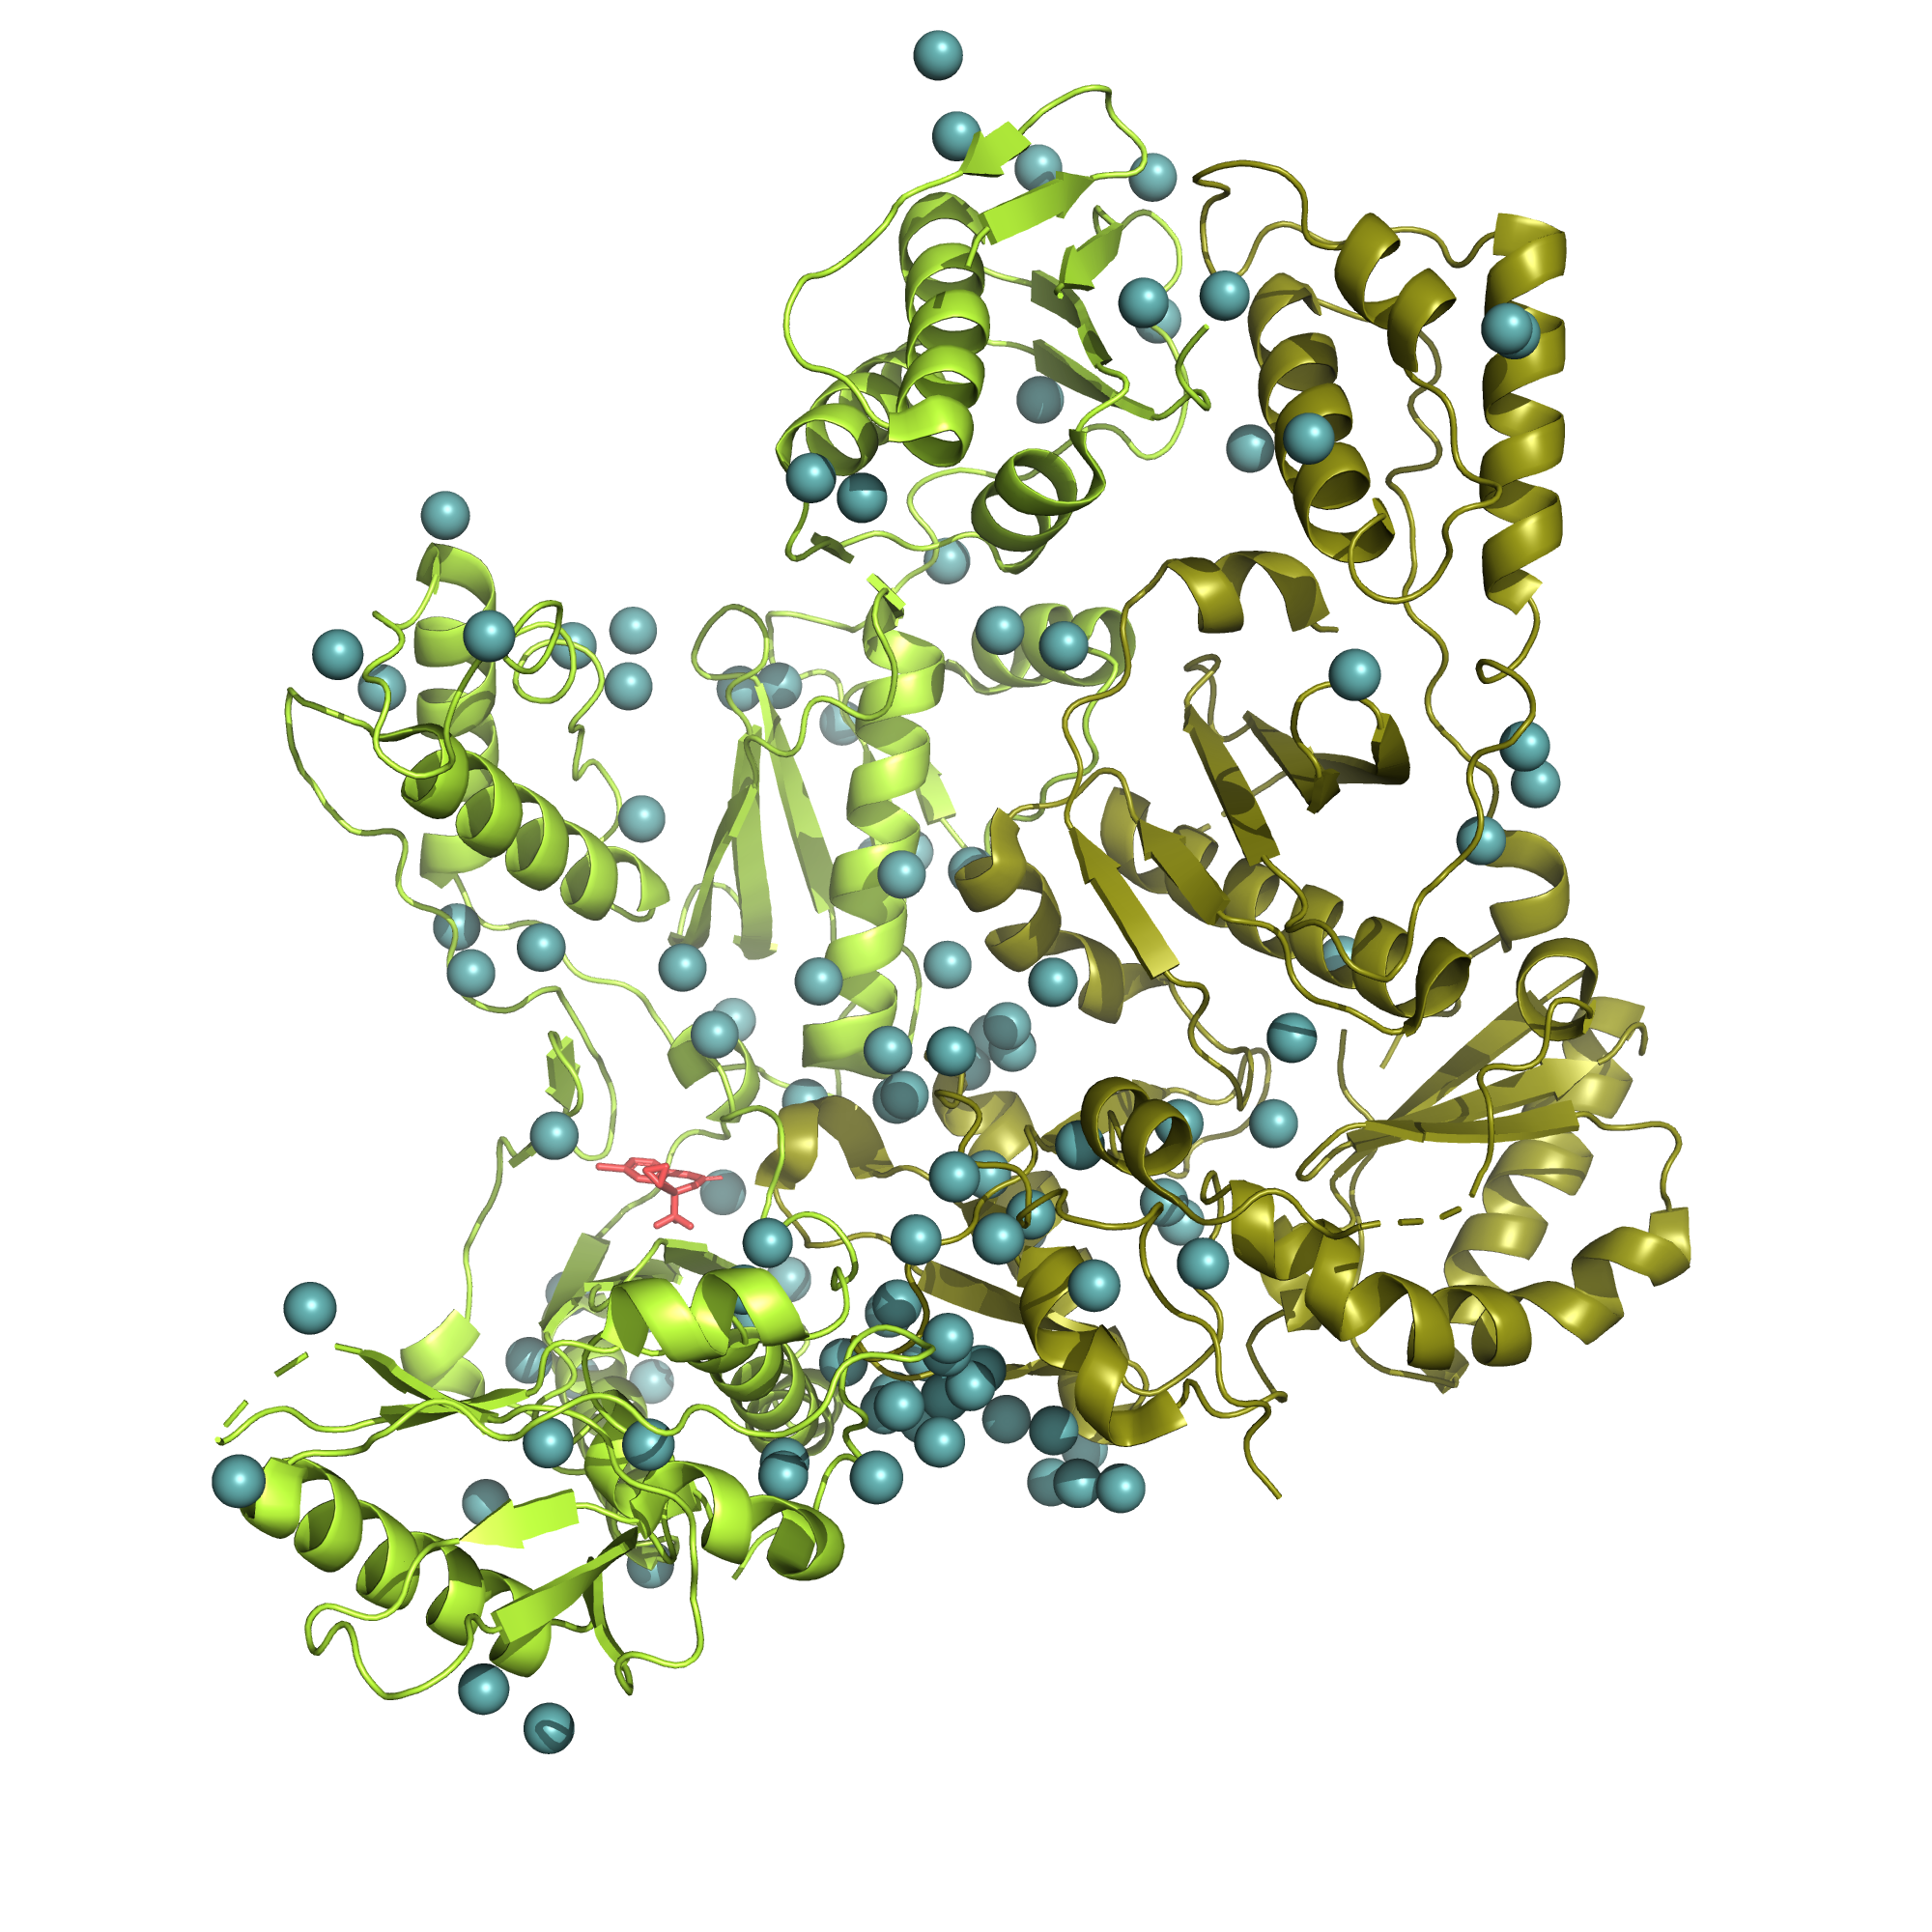
\includegraphics[width=0.5\textwidth]{../figures/water.png}
    \caption{Protein complex, water molecules are represented by the blue beads according to the VdW radius, via \cite{pymol} \label{fig:total}}
\end{figure}

\subsection{Model preparation}
Since the two residues (CSD and EFZ) were not associated to any force field, the parameters were manually added through model preparation.
Steps followed for such procedures were the same for both the residues, involving these procedures:

\begin{itemize}
    \item Hydrogen addition
    \item Charges computation
    \item General force field (gaff) assignment
\end{itemize}

After these procedures, the final parameters were saved in a .lib file ready to be loaded for the final simulation process. The model preparation allowed so to integrate the different parts of the macromolecule and solute it with the tip3 library.  

Given this initial modelization it was decided to study the behaviour of two particular configurations:
\begin{itemize}
    \item Chain A + EFZ
    \item Chain B + EFZ
\end{itemize}
This was done to ease computations with a smaller set of elements to simulate, while having the possibility to study reciprocal behavior of the EFZ residue and the active residues of both proteins. Active residue were in particular individuated using Pymol\cite{pymol}, by individuating the residues closer than 4 \AA to EFZ in both the chains.

\begin{figure}
    \centering
    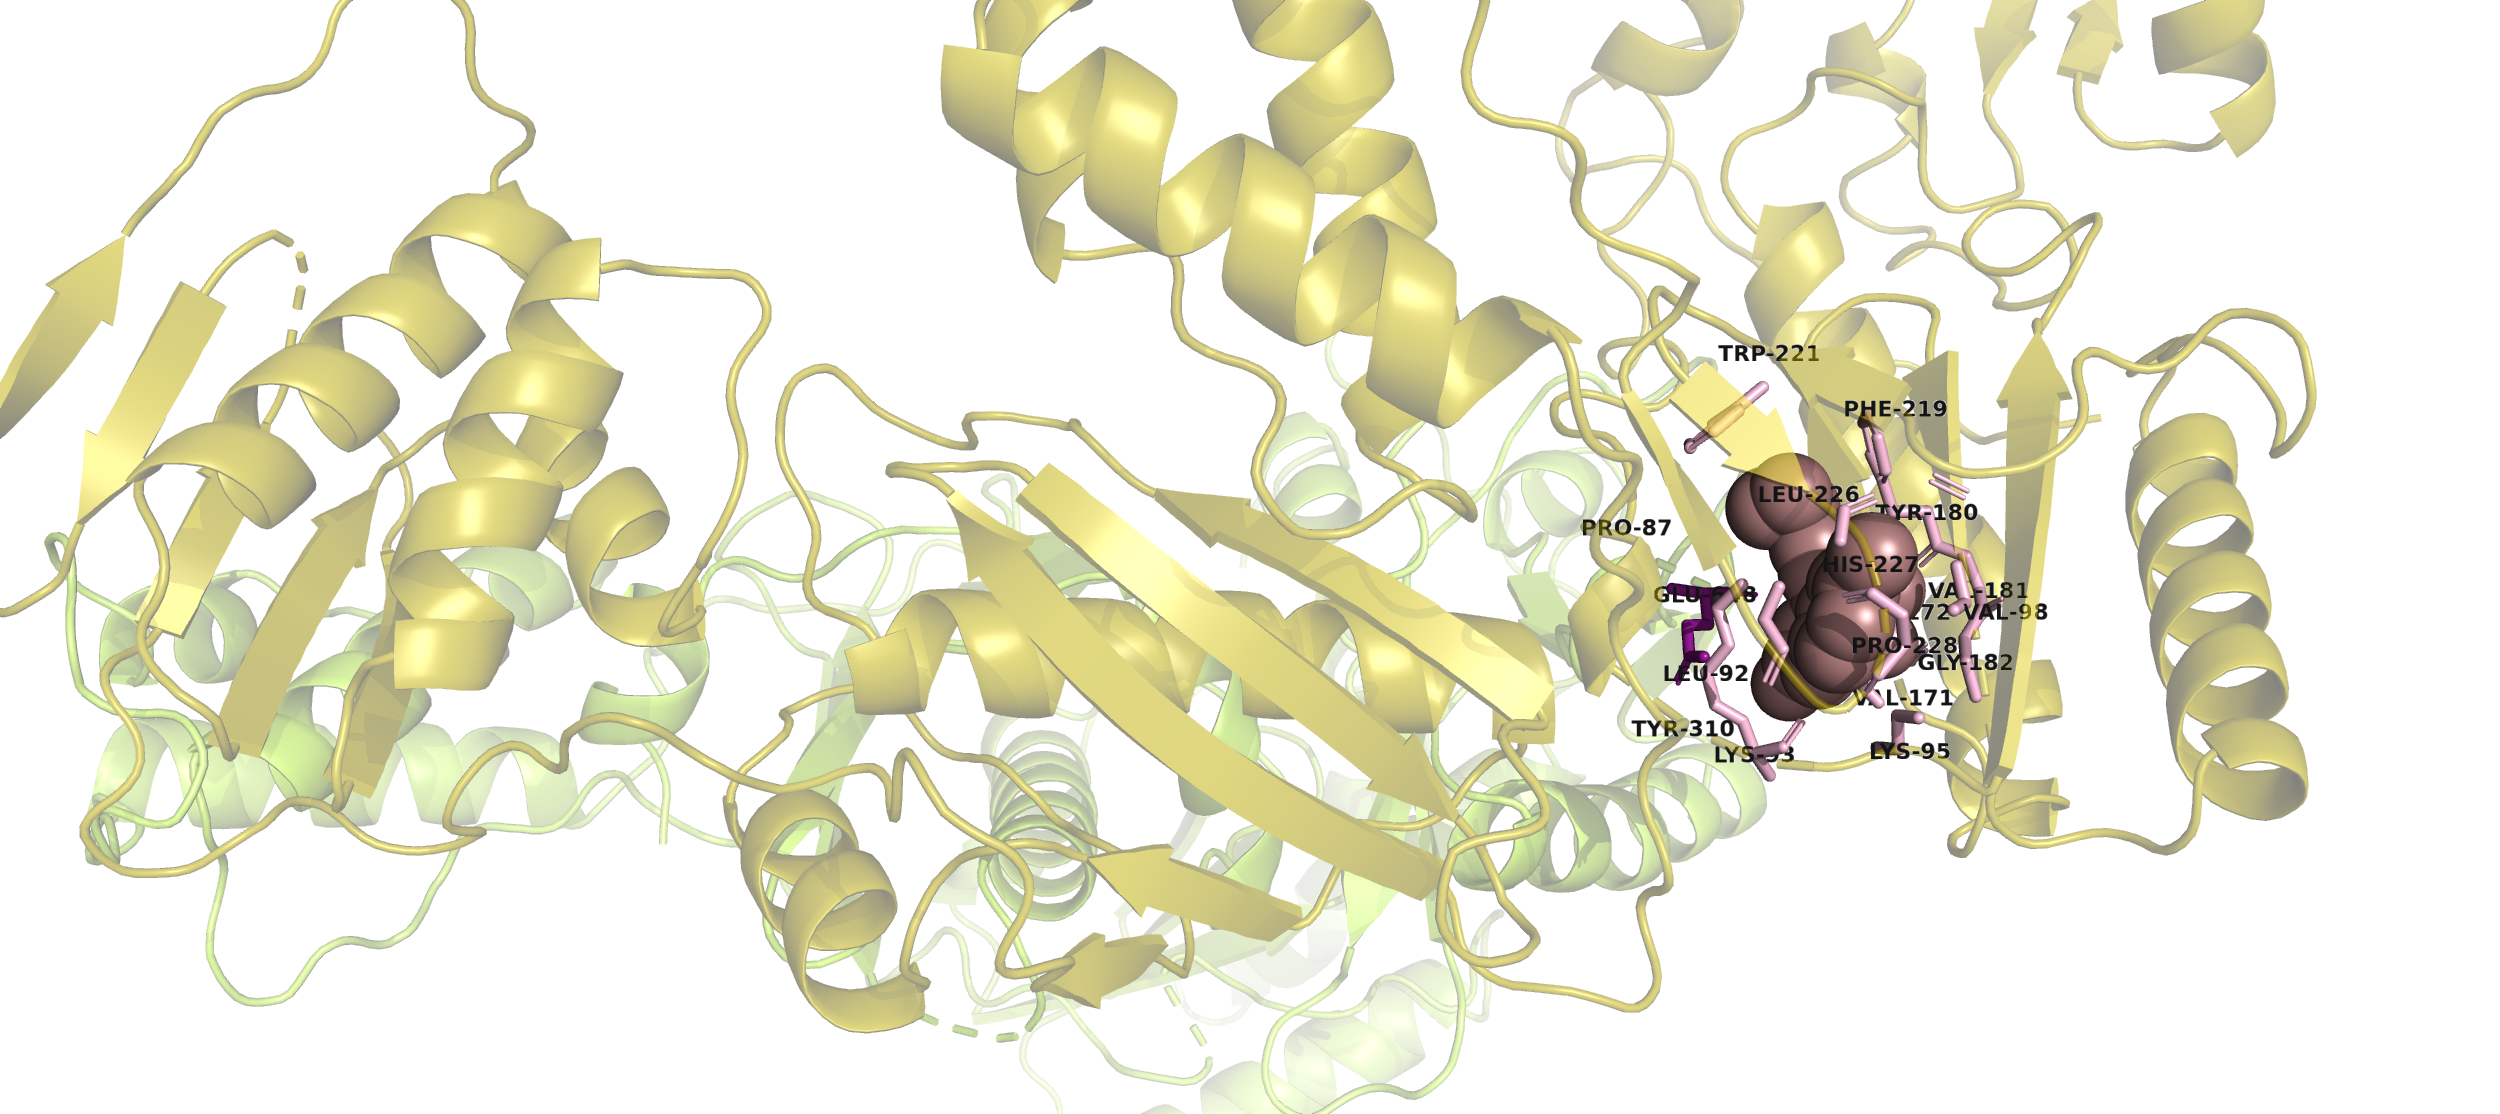
\includegraphics[width=\textwidth]{../figures/act_res.png}
    \caption{Labelled active residues found in the proximity of EFZ (Brown beads)\label{fig:sample}}
\end{figure}
In total were found 15 active residues in the chain A, and a single one in the chain B. These residues will be then considered during
analysis to study the water distribution around active sites.

Before any action was taken, the newly-generated pdb files underwent some cleaning through the command pdb4amber, and was then optimized for a rectangular box through simulaid \cite{simulaid}. After this first optimization it was possible to use tleap, load the pdb file corresponding to each tested configuration and define the force fields using predefined libraries ("ff99SB") and user-defined ones for the CSD and EFZ residues. In this last phase some warnings were raised by tleap concerning improper tension terms, but nothing able to influence the operation result.

\subsection{Solvent addition and minimization}
After having prepared the model for the two sistems to simulate, preequilibrated water was added using "TIP3" library of tleap using a rectangular box with minimum distance from solvate fixed at 12 \AA. Ions were also added to the system to neutralise the charges, that were equal to +6 in the Chain B + EFZ case, and equal to -2 in the Chain A + EFZ case.
These charges were balanced with respectively 6 Cl- ions in the first case, and 2 Na+ ions in the latter one. Errors agains were raised by tleap, but were similar to the ones found during the loading phase.

Given this initial configuration it was possible to start a minimization routine using periodic boundary conditions along 2000 iterations with a cut fixed at 15 \AA. This last process allowed to retrieve a stable configuration, moving from starting energies equal to $E=1.5\cdot 10^{13}$ for the Chain A + EFZ case and $E=-1.1\cdot 10^{5}$ for che Chain B + EFZ to respectively energies equal to $E=-3.4\cdot 10^{5}$ and $E=-2.6\cdot 10^{5}$.

\begin{figure}
    \centering
    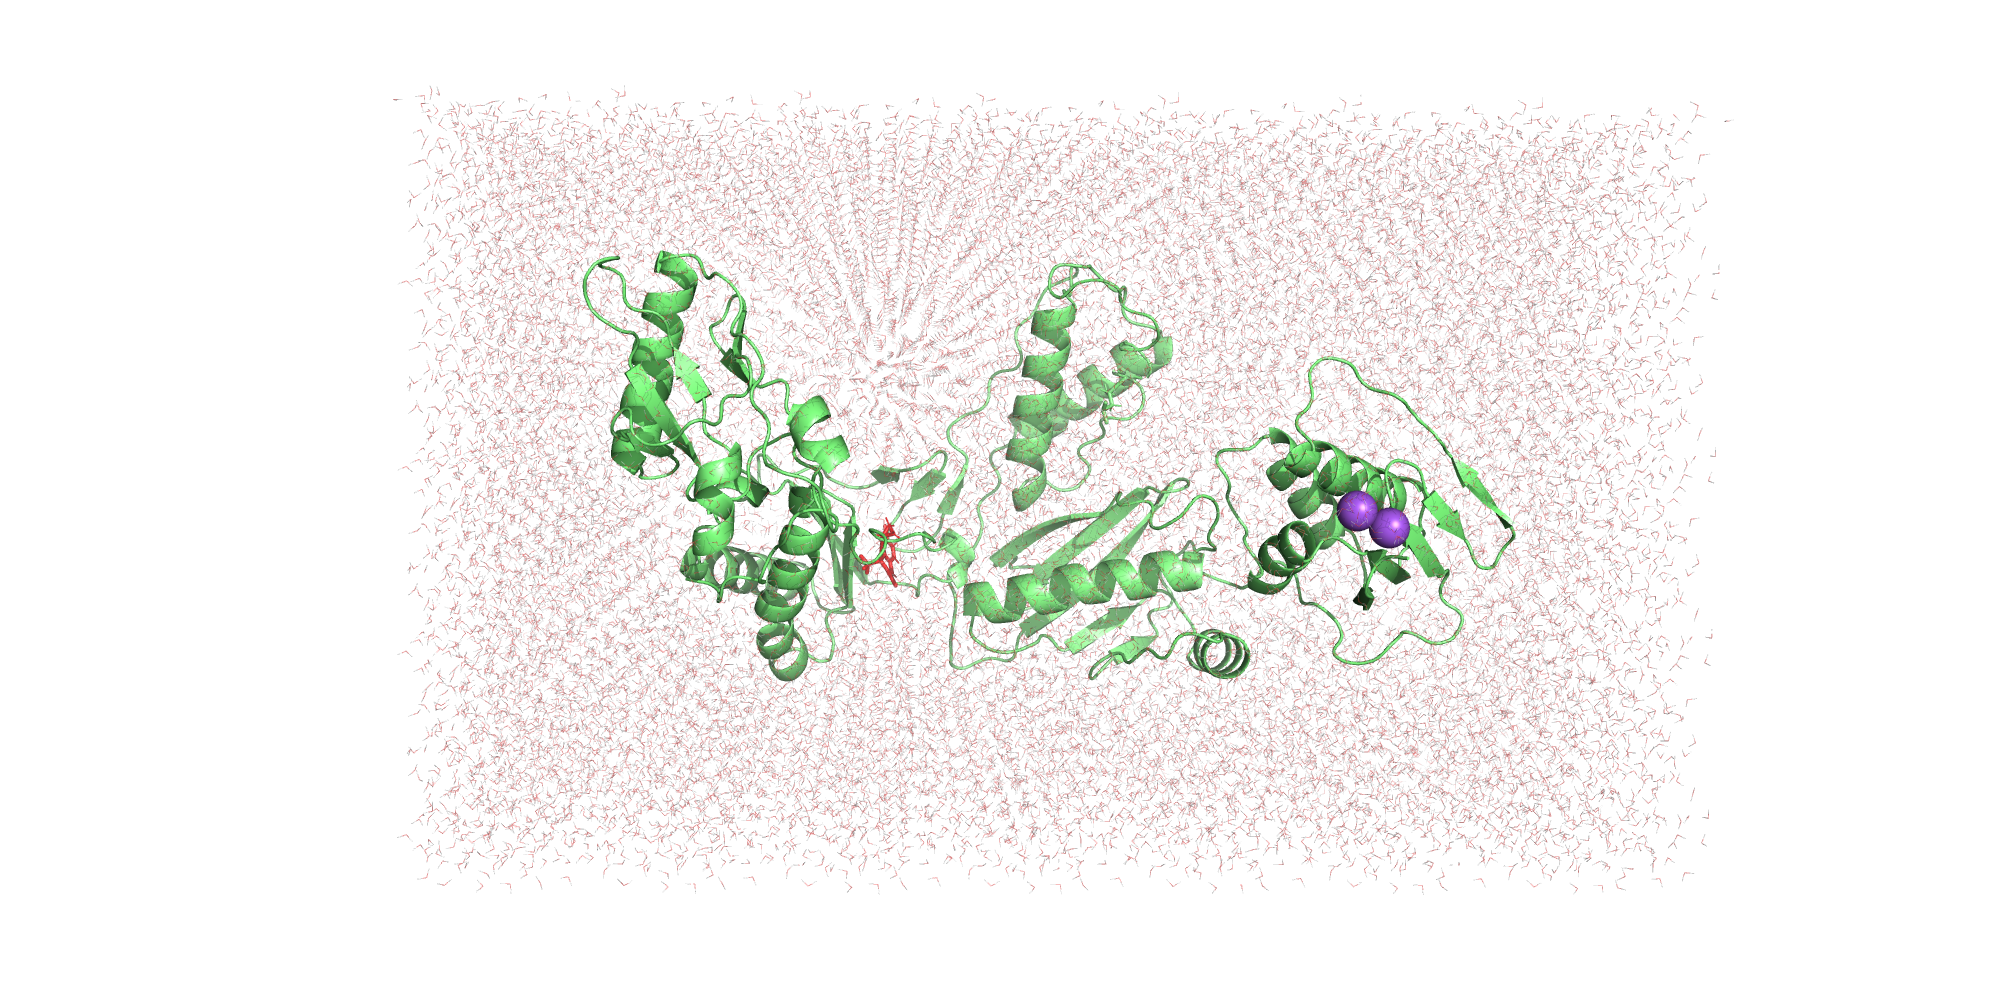
\includegraphics[width=0.7\linewidth, clip, trim= 200 20 160 20]{../figures/chain_a_efz_solv.png}
    \caption{Chain A+ EFZ configuration in solution after minimization. In red can be seen the EFZ residue, while the purple beads represent the Na+ ions.\label{fig:chain_a_efz_solv}}
\end{figure}

\begin{figure}
    \centering
    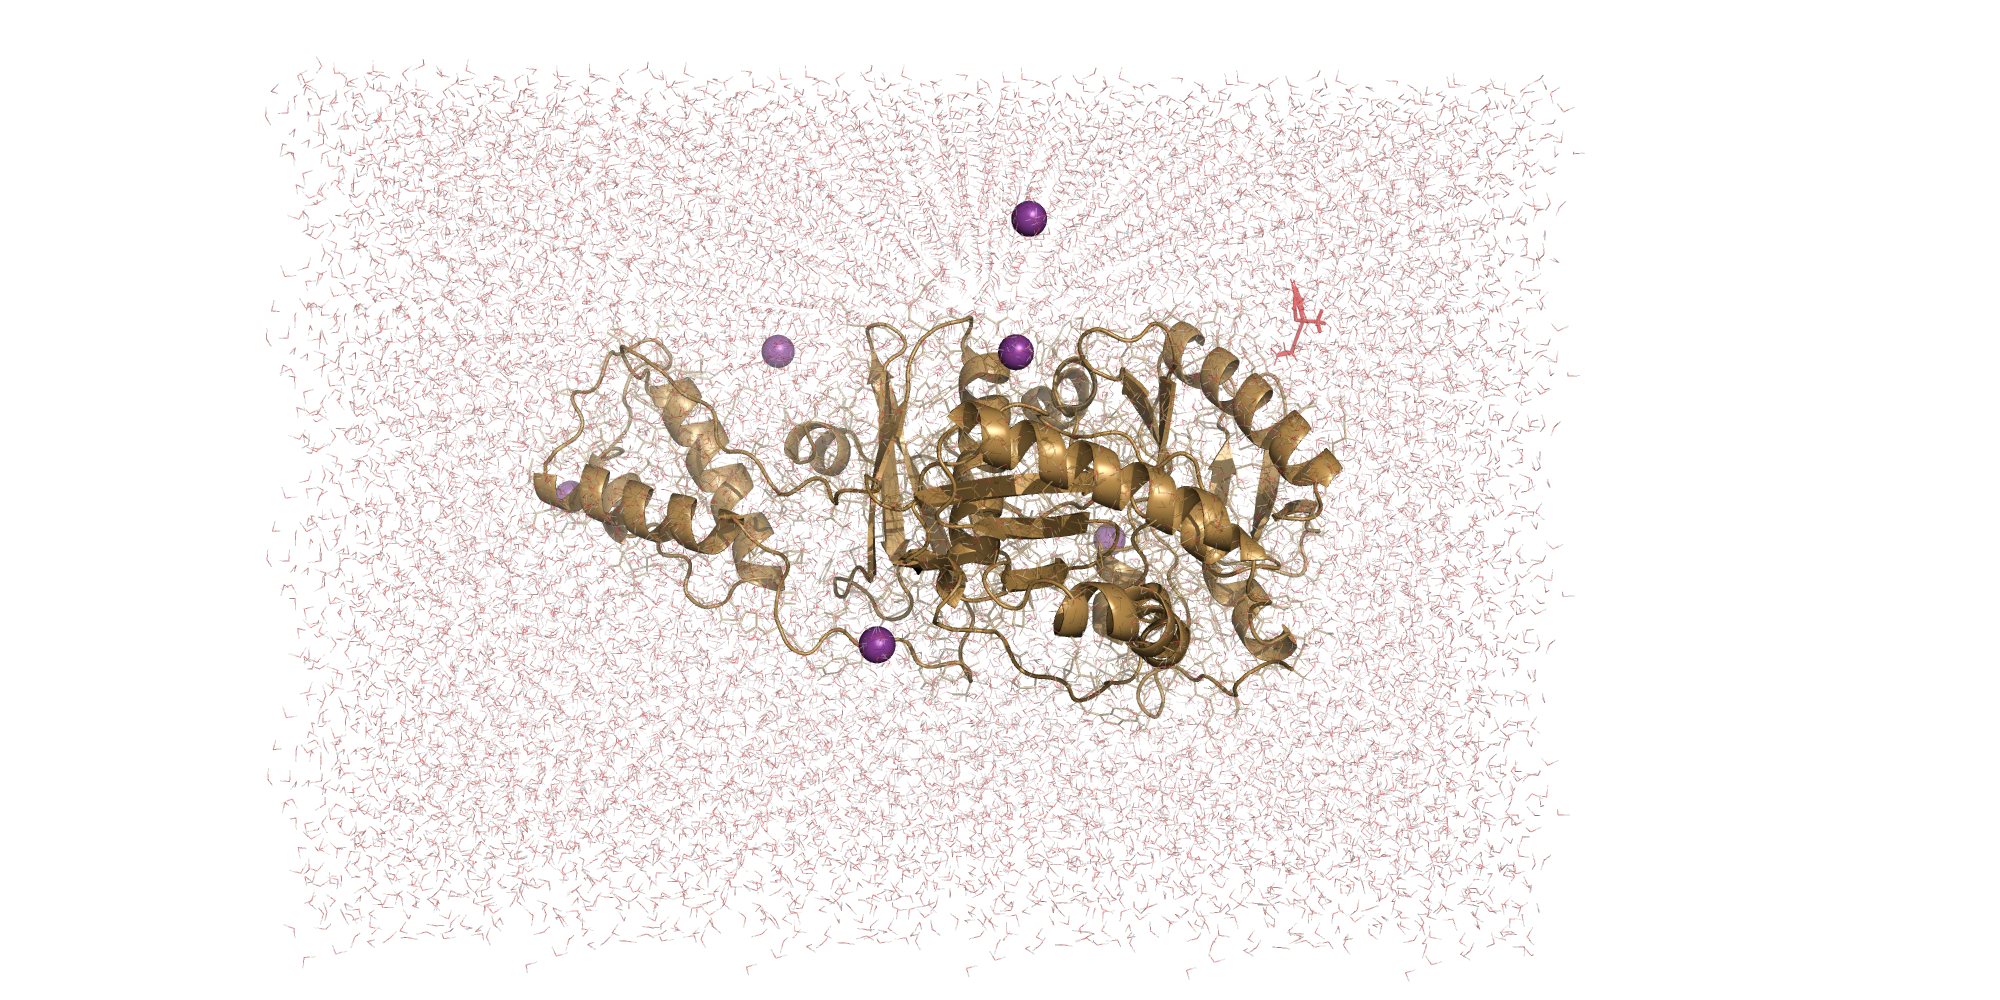
\includegraphics[width=0.7\linewidth, clip, trim= 135 20 180 20]{../figures/chain_b_efz_solv.png}
    \caption{Chain B + EFZ configuration in solution after minimization. In red can be seen the EFZ residue, while the purple beads represent the Cl- ions.\label{fig:chain_b_efz_solv}}
\end{figure}

\subsection{Molecular dynamics}
The minimized configuration does not have any assigned speed, that has so to be assigned by fixing an initial temperature and extracting them randomly from the Boltzmann distribution. Using a second script the system, starting from this initial configuration, was heaten up in periodic boundary conditions from an initial temperature of 0 K, to a final temperature of 298 K. This was done in an isothermic and isobaric esemble coded using a langevin thermostat. Along with these settings the cut was again fixed at 15 \AA, while the hydrogen movement was constrained with a harmonic potential.
The heating procedure was finally carried out in 10000 steps, each one of 2 fs, thanks to the fixed constraints. This allowed in both cases to reach the required temperature without fluctuations larger than a few degrees.


After having heaten up the system it was possible to perform so the actual molecular simulation and study the system at a fixed temperature. A simulation with the same settings of the one discussed for the heating was so set up, with the temperature fixed at 298 K as before.
Again, thanks to the Langevin thermostat it is possible to keep almost fixed the temperature around the required value, with a RMS that can be found to be around 1 to 2 degrees in both the tests done.

\subsection{Analysis methods}
The main interest of these simulations is to study and discuss the behaviour of water molecules and active residues during the simulation. To do so two software utilities were used:
\begin{itemize}
    \item VMD\cite{VMD}, to calculate the radial distribution function g(r)
    \item MDTraj\cite{MDTraj}, to study the trajectory of the simulated structure.
\end{itemize}

Both these tools refer to the following formulas:

$$g(r) = \frac{V}{4\pi r^2 \Delta r N^2}\sum_i n_i(r,\Delta r) \quad n_i = \mathrm{number \, of \, atoms \, in \, the \, \{r,\Delta r\} \, shell}$$
 
$$K(r) = 4\pi \rho \int_{0}^{r_c} dr r^2 g(r)$$

Both these formulas are discretized by dividing the distance domain in intervals of length equal to 0.1 \AA.

Along with these analyses were considered also the calculation of RSMD of the global complex and the RSMF of the EFZ residue. The first computation allows so to determine how much the protein's residues moves from the starting configuration during the simulation, by computing the mean deviation from the reference. The latter one instead allows understanding how much a single residue fluctuates from a reference configuration.
\section{Results}

\subsection{Radial distribution function and coordination number}
The first calculation was done to compute the radial distribution function g(r), in order to understand the local distribution of water molecules around the active sites and the EFZ ligand. The calculation was done taking into account the periodic boundary conditions, allowing to calculate over distances much larger than the 12 \AA of the solvation box.

\begin{figure}
    \centering
    \includegraphics[width=\textwidth]{../figures/a_chain_act.pdf}
    \caption{Radial distribution function g(r) and running coordination number K(r) of water around active sites for the configuration Chain A + EFZ\label{fig:gofr_chain_a_efz}}
\end{figure}

Only a few residues show a significative local structure, for example the residue 93, showing a hydration cell around
5 \AA, or the residue 228, with a similar behaviour and local fluctuations probably associated to more dense shells.
Around residues like 310,180 and 98 it is possible to observe such similar structures, indicating small conglomerates of water molecules. The other residues have in general more repulsive behaviours, including EFZ, with a shape increasing continuosly with the increase in distance.

\begin{figure}
    \centering
    \includegraphics[width=\textwidth]{../figures/b_chain_act.pdf}
    \caption{Radial distribution function g(r) and running coordination number K(r) of water around active sites for the configuration Chain B + EFZ\label{fig:gofr_chain_b_efz}}
\end{figure}

In the second tested configuration results are very similar, with the residue EFZ having a less repulsive behaviour, but the same continuos increase with distance. Residue 129 instead has two clear hydration cells between 0 and 5 \AA.

For the coordination numbers the only difference between different residues is related to the repulsivity, and reflects on the initial plateau, noticeable before the main increasing trend.

\subsection{RMSF and RMSD}
% \subsection{RMSD and RMSF}
% \begin{figure}[H]
%     \centering
%     \includegraphics[width=0.5\textwidth]{../figures/rmsd.pdf}
%     \caption{RSMD of the global complexes for the Chain A + EFZ case (left) and the Chain B + EFZ case (right)\label{fig:rmsd}}
% \end{figure}

% \subsection{RMSD and RMSF}
% \begin{figure}[H]
%     \centering
%     \includegraphics[width=0.5\textwidth]{../figures/rmsf_efz.pdf}
%     \caption{RSMF of the EFZ residue for the Chain A + EFZ case (left) and the Chain B + EFZ case (right)\label{fig:rmsd}}
% \end{figure}
\section{Conclusions}
\section{Code}
All the code used in this project and its outputs can be found at this \href{https://github.com/Confizolo/PoDProjects}{link}, in the MS directory.
\bibliographystyle{plain} % We choose the "plain" reference style
\bibliography{bibl} % Entries are in the refs.bib file

\end{document}
